\section{Introduction}\label{sec:intro}

Population health research is becoming increasingly based on data-driven methods
(as opposed to those designed solely by clinical experts) for patient-centred
care through the advent of accessible software and a relative abundance of
electronic data. Population health research concerns itself with better
understanding the healthcare needs and behaviours of a population, so to further
that end it can be helpful to find an appropriate segmentation of that
population; such a segmentation allows for finer-grained analysis of groups in
the population that share some form of homogeneity. One commonly used method for
such patient-centred analysis is that of patient flow and their interaction with
the healthcare system.

However, this process relies heavily on detailed data --- about both the system
and the population within that system --- which may limit research where
sophisticated data pipelines are not yet in place. This work demonstrates how
this issue may be overcome using administrative, spell-level hospital data to
build a patient clustering that feeds into a multi-class queuing model.
Specifically, this work examines patient records from the NHS Wales Cwm Taf
Morgannwg University Health Board (UHB) that present chronic obstructive
pulmonary disease (COPD). COPD is of particular interest to Cwm Taf Morgannwg as
it was found that they had the highest prevalence of the condition across all
the Welsh health boards in an internal report by NHS Wales.

% TODO No reference for graph sent by Kendal but is this alright?

% TODO Image of process: administrative data -> extract service parameters ->
%                        validate parameters with Wasserstein distance ->
%                        continue with queuing model as normal

\subsection{Literature review}\label{subsec:review}

Clustering is the process of separating the instances of a dataset into distinct
parts to maximise homogeneity within each cluster and heterogeneity between each
cluster. Within healthcare, and particularly population health, this concept has
many applications. When applying this to a population, some form of patient
corpus is considered the \emph{de facto} dataset but the choice of
characteristics with which to describe a patient or record remains open. The
review for this work identified three groups of characteristics used to cluster
a patient population: a patient's system utilisation metrics, their clinical
attributes and their pathway. The first two belong to a method known as
segmentation analysis wherein a patient population is segmented in the
straightforward sense. The latter, however, does not strictly segment the
patients directly but rather groups their movements through a healthcare system
via process mining.~\cite{AG2018}~and~\cite{DDGM+12015} demonstrate how this
technique can help to improve the efficiency of a hospital system rather than
tackling the issue of patient-centred care as is the focus of this work.

Segmentation analysis is an expanding part of population health literature as it
allows for the targeted analysis of heterogeneous datasets and simplified
communication of patient needs to stakeholders within a healthcare
system~\cite{VMD2016review, YKTT+12018}. For instance, profiling often forms
part of segmentation analysis where each segment can be summarised in a phrase
or infographic~\cite{VMD2016, YSKT+42019}.

% TODO Brief literature review of:
%       - clustering patient corpus
%       - reverse-engineering model parameters in healthcare ???
%       - queuing in healthcare

\subsection{Cluster analysis}\label{subsec:clusters}

\begin{table}
    \centering
    \resizebox{\textwidth}{!}{%
        \begin{tabular}{lllllll}
\toprule
               &        &   Cluster &             &            &           & Population \\
               &        &         0 &           1 &          2 &         3 &            \\
\midrule
\textbf{Characteristics} & \textbf{Percentage of spells} &   9.90701 &     19.2708 &    69.3859 &   1.43633 &        100 \\
               & \textbf{Mean spell cost, £} &   8051.23 &     2309.63 &    1508.41 &   17888.4 &     2265.4 \\
               & \textbf{Percentage of recorded costs} &   29.0137 &     19.3806 &    48.2048 &   3.40094 &        100 \\
               & \textbf{Mean COPD adm. in last year} &   2.19331 &     1.96464 &     1.8819 &   2.08974 &    1.93168 \\
               & \textbf{Minimum LOS} &   12.8229 & -0.00486111 & -0.0208333 &   48.8174 & -0.0208333 \\
               & \textbf{Mean LOS} &   25.3024 &     6.46379 &    4.10628 &   75.3601 &    7.68393 \\
               & \textbf{Maximum LOS} &   51.3604 &      30.859 &     16.941 &   224.928 &    224.928 \\
               & \textbf{Median no. of LTCs} &         2 &           3 &          1 &         3 &          1 \\
               & \textbf{Median no. of ICDs} &         9 &           8 &          5 &        11 &          6 \\
               & \textbf{Median CCI} &         9 &          20 &          4 &        18 &          4 \\
\textbf{Intervention prevalence} & \textbf{None, \%} &   80.2045 &     83.4209 &    65.7643 &   89.7436 &    70.9419 \\
               & \textbf{PR, \%} &   15.7993 &     13.4257 &    27.9724 &   8.97436 &    23.6903 \\
               & \textbf{SN, \%} &   3.81041 &      2.8667 &     4.6311 &   1.28205 &    4.16168 \\
               & \textbf{Both, \%} &  0.185874 &     0.28667 &    1.63217 &         0 &    1.20615 \\
\textbf{LTC prevalence} & \textbf{Pulmonary disease, \%} &       100 &         100 &        100 &       100 &        100 \\
               & \textbf{Diabetes, \%} &    19.052 &     28.1414 &    14.8355 &        25 &    17.9634 \\
               & \textbf{AMI, \%} &   13.8476 &     22.9336 &    8.75796 &   16.0256 &    12.0983 \\
               & \textbf{CHF, \%} &   12.4535 &     53.8462 &          0 &   26.2821 &    11.9878 \\
               & \textbf{Renal disease, \%} &   7.52788 &     19.5413 &     1.9241 &   17.9487 &    6.10441 \\
               & \textbf{Cancer, \%} &   7.62082 &     12.2312 &    2.93259 &   10.8974 &    5.30338 \\
               & \textbf{Dementia, \%} &   6.87732 &     21.2613 &          0 &   26.9231 &    5.16527 \\
               & \textbf{CVA, \%} &   8.64312 &     13.3301 &   0.703291 &   19.8718 &    4.19851 \\
               & \textbf{PVD, \%} &   4.36803 &     7.69231 &    2.26911 &   5.76923 &    3.57242 \\
               & \textbf{CTD, \%} &   5.11152 &     4.25227 &     3.1051 &   4.48718 &    3.54479 \\
               & \textbf{Obesity, \%} &   2.50929 &     3.01003 &     1.4862 &   7.69231 &    1.97035 \\
               & \textbf{Metastatic cancer, \%} &   1.57993 &     4.49116 &          0 &  0.641026 &    1.03121 \\
               & \textbf{Paraplegia, \%} &   1.30112 &     3.72671 &   0.238854 &  0.641026 &    1.02201 \\
               & \textbf{Diabetic compl., \%} &  0.185874 &     0.86001 &   0.477707 &   1.92308 &   0.543228 \\
               & \textbf{Peptic ulcer, \%} &   1.57993 &    0.812231 &   0.225584 &   1.28205 &   0.487985 \\
               & \textbf{Sepsis, \%} &    1.7658 &    0.907788 &   0.145966 &   1.92308 &   0.478777 \\
               & \textbf{Liver disease, \%} &   0.27881 &    0.477783 &   0.225584 &         0 &   0.276218 \\
               & \textbf{C. diff, \%} &  0.743494 &   0.0955566 &  0.0132696 &  0.641026 &   0.110487 \\
               & \textbf{Severe liver disease, \%} &  0.185874 &    0.430005 &          0 &         0 &    0.10128 \\
               & \textbf{MRSA, \%} &   0.27881 &   0.0477783 &  0.0265393 &   1.28205 &   0.073658 \\
               & \textbf{HIV, \%} &         0 &           0 &  0.0265393 &         0 &  0.0184145 \\
\bottomrule
\end{tabular}

    }\caption{A summary of patient-level clinical attributes and disease
    prevalence by cluster and by population}\label{tab:summary}
\end{table}

\begin{figure}
    \centering
    \begin{subfigure}{\halfimgwidth}
        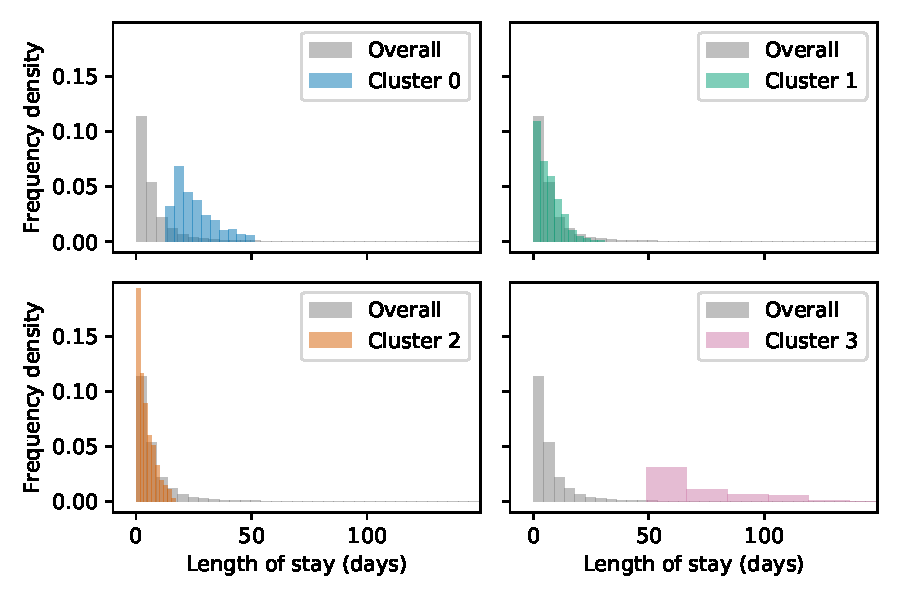
\includegraphics[width=\linewidth]{cluster_los}
        \caption{}\label{fig:cluster_los}
    \end{subfigure}\hfill%
    \begin{subfigure}{\halfimgwidth}
        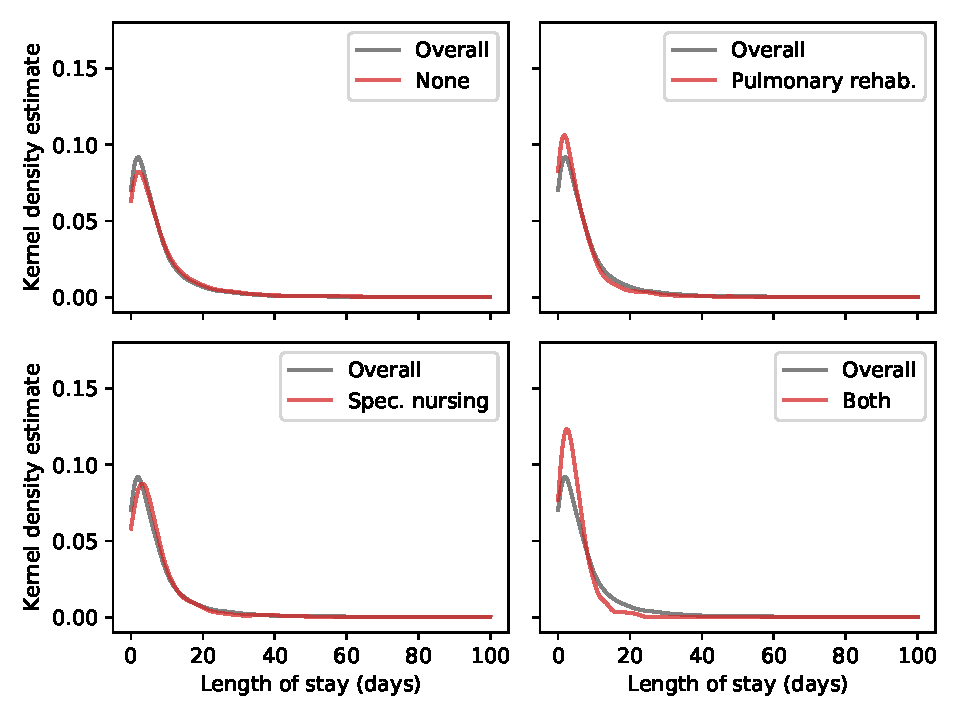
\includegraphics[width=\linewidth]{intervention_los}
        \caption{}\label{fig:intervention_los}
    \end{subfigure}
    \caption{%
        Kernel density estimate plots for length of stay by
        (\subref{fig:cluster_los}) cluster and (\subref{fig:intervention_los})
        intervention
    }\label{fig:los_kde}
\end{figure}

\begin{figure}
    \centering
    \begin{subfigure}{\halfimgwidth}
        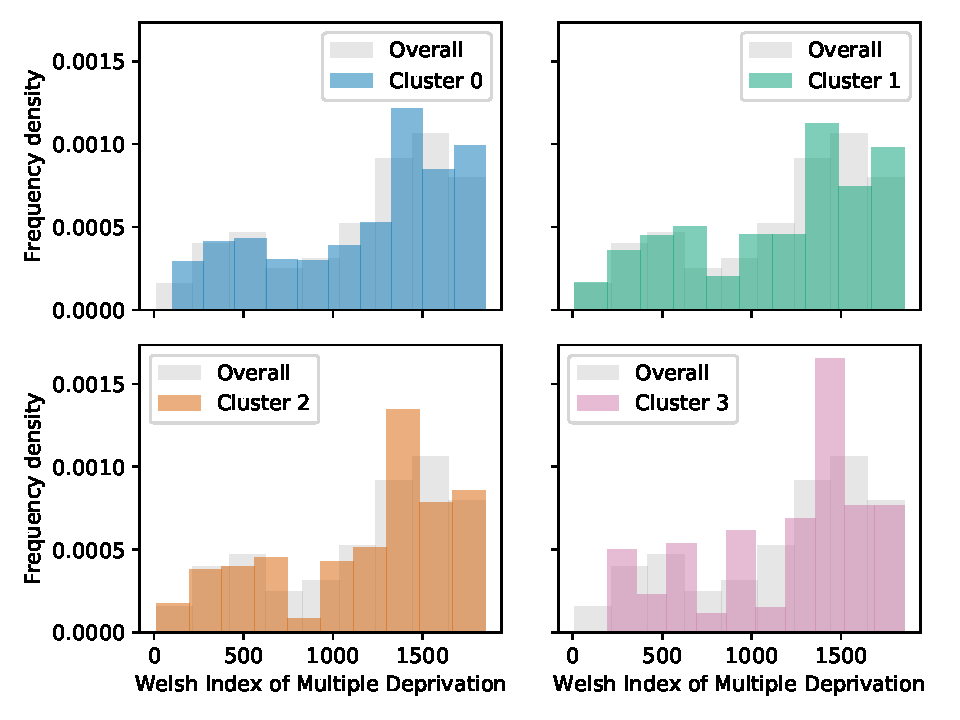
\includegraphics[width=\linewidth]{cluster_wimd}
        \caption{}\label{fig:cluster_wimd}
    \end{subfigure}\hfill%
    \begin{subfigure}{\halfimgwidth}
        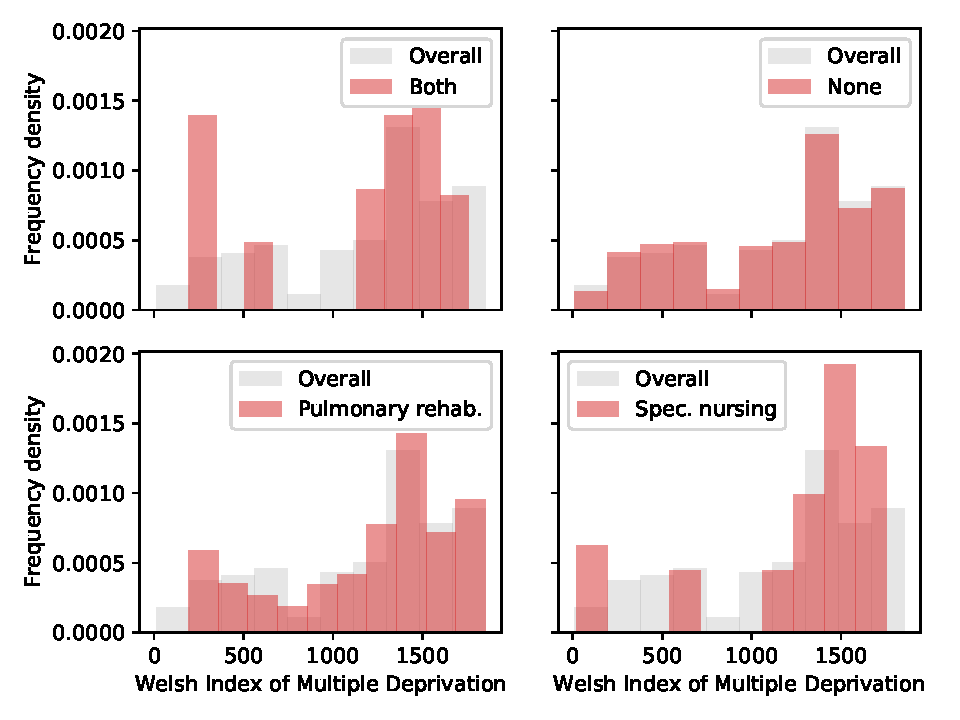
\includegraphics[width=\linewidth]{intervention_wimd}
        \caption{}\label{fig:intervention_wimd}
    \end{subfigure}
    \caption{%
        Histograms for WIMD by (\subref{fig:cluster_wimd}) cluster and
        (\subref{fig:intervention_wimd}) intervention
    }\label{fig:wimd_hist}
\end{figure}

\begin{figure}
    \centering
    \begin{subfigure}{\halfimgwidth}
        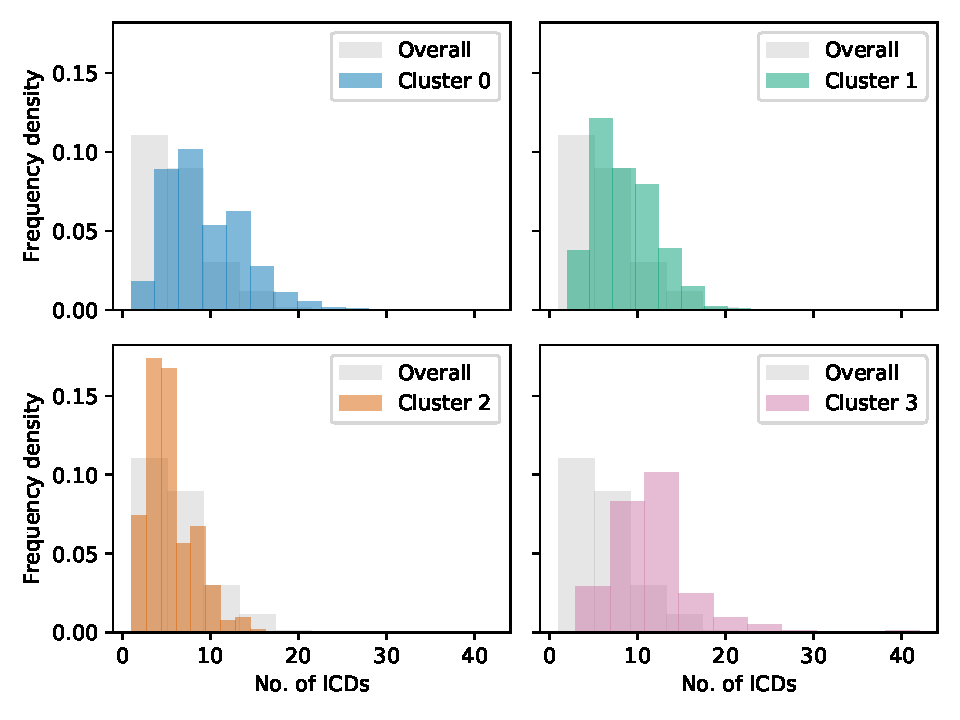
\includegraphics[width=\linewidth]{cluster_n_icds}
        \caption{}\label{fig:cluster_n_icds}
    \end{subfigure}\hfill%
    \begin{subfigure}{\halfimgwidth}
        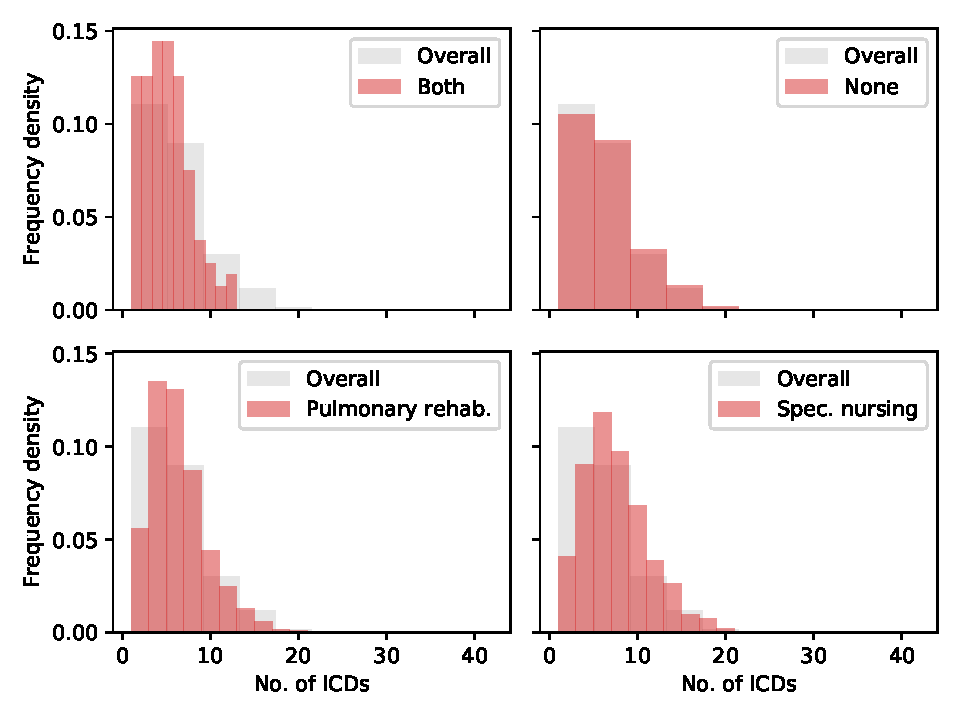
\includegraphics[width=\linewidth]{intervention_n_icds}
        \caption{}\label{fig:intervention_n_icds}
    \end{subfigure}
    \caption{%
        Histograms for number of ICDs by (\subref{fig:cluster_n_icds}) cluster
        and (\subref{fig:intervention_n_icds}) intervention
    }\label{fig:n_icds_hist}
\end{figure}

\begin{figure}
    \centering
    \begin{subfigure}{\halfimgwidth}
        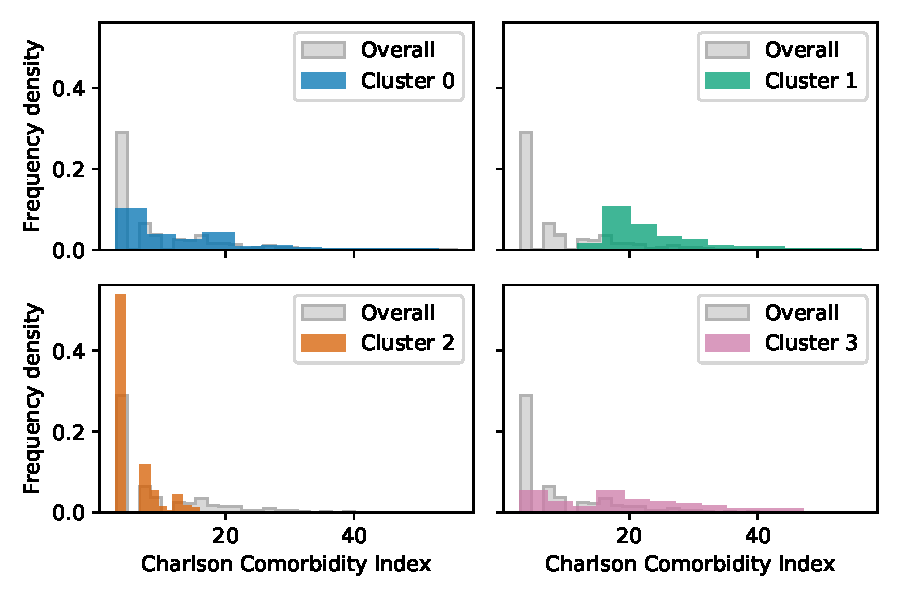
\includegraphics[width=\linewidth]{cluster_charlson_gross}
        \caption{}\label{fig:cluster_charlson}
    \end{subfigure}\hfill%
    \begin{subfigure}{\halfimgwidth}
        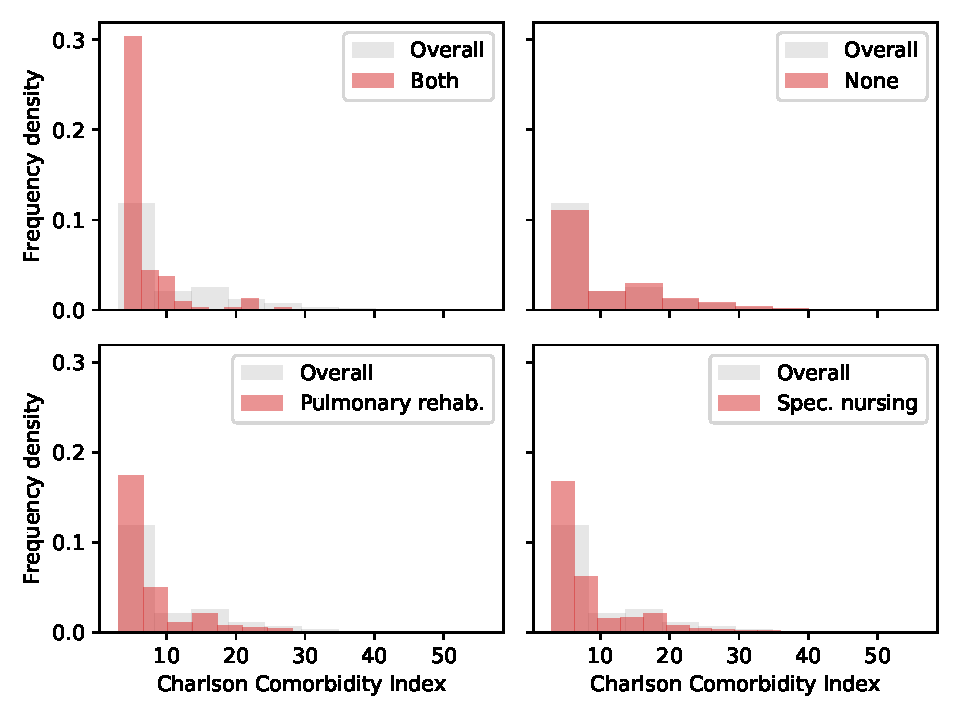
\includegraphics[width=\linewidth]{intervention_charlson_gross}
        \caption{}\label{fig:intervention_charlson}
    \end{subfigure}
    \caption{%
        Histograms for CCI by (\subref{fig:cluster_charlson}) cluster and
        (\subref{fig:intervention_charlson}) intervention
    }\label{fig:charlson_hist}
\end{figure}


% TODO Condensed analysis of clustering
%       - choosing k and a clustering algorithm
%       - comparison with treatment segmentation
